\documentclass{article}
\usepackage{comment}        % for comment
\usepackage[utf8]{inputenc} % for Chinese
\usepackage{CJKutf8}        % for Chinese words
\usepackage{fancyhdr}       % for header and footer
\usepackage{enumerate}      % for enumerate
\usepackage{enumitem}       % for enumerate label bold
\usepackage{amssymb}        % for math notations
\usepackage{amsthm}         % for proofs
\usepackage{mathtools}      % for math notations
\usepackage{graphicx}       % for graphics
\usepackage[left=1.9cm, right=1.9cm, top=2.54cm, bottom=2.54cm]{geometry} %set margin
\renewcommand{\baselinestretch}{1.1} % 行距
\usepackage{graphicx}
\newcommand{\argmin}{\mathop{\mathrm{argmin}}}

\pagestyle{fancy}
\fancyhf{}
\rhead{\thepage}
\lhead{Machine Learning Techniques (108-2)}

\begin{document}
\begin{CJK*}{UTF8}{bsmi}
    \begin{center}
        \begin{Large} \textbf{Homework \#1} \end{Large}
        \\[10pt]
        \begin{large} B07902028 \enspace 資工二 \enspace 林鶴哲 \end{large}
    \end{center}
    \begin{normalsize}
    \begin{enumerate}[label=\textbf{\arabic*}.]
        \item We compute each $\mathbf{z}(\mathbf{x})$ and plot the transformed vectors, by easy observation, one can see that $z_1 = -0.5$ is the optimal hyperplane line on $\mathcal{Z}$ space.
        \begin{center} \includegraphics[scale = 0.65]{p1.png}
        \end{center}
        
        \item The standard form of a QP problem can be written as
        \[ \begin{aligned} \min_{\mathbf{x}}\enspace \enspace &  \frac{1}{2}\mathbf{x}^TP\mathbf{x} + q^T\mathbf{x}\\
        \text{subject to \enspace \enspace}& G\mathbf{x} \le h\\
        &A\mathbf{x} = b\end{aligned}\]
        Let $N = 7$, we set the optimization as follows:
        \begin{itemize}
            \item $P_{ij} = y_iy_jK(\mathbf{x_i}, \mathbf{x_j})$ for $1 \le i, j \le N$, $q = \mathbf{-1}_N$.
            \item $G_i = - \text{(the i-th unit vector)}$ for $1 \le i \le N$, $h = \mathbf{0}_N$
            \item $A = \mathbf{1}_N$, $b = 0$
        \end{itemize}
        Then use \verb|cvxopt| package in python, we obtain the optimal $\alpha = (0.000,0.704,0.704,0.889,0.259,0.259,0.000)$.
        Based on the nonzero $\alpha_i$, we know that there are 5 support vectors: $\mathbf{x_2}, \mathbf{x_3}, \mathbf{x_4}, \mathbf{x_5}$ and $\mathbf{x_6}$.
        
        \item Let $\mathbf{x}^T = \begin{bmatrix}x_1&x_2 \end{bmatrix}$, the curve can be written as
        \[ \Gamma: \mathbf{w}^T\Phi(\mathbf{x})+ b = 0 \]
        where
        \[ \begin{aligned} \mathbf{w}^T\Phi(\mathbf{x}) = \sum_{\text{SV}}\alpha_n y_n \mathbf{z_n}^T \Phi(\mathbf{x}) = \sum_{\text{SV}}\alpha_n y_n K(\mathbf{x}, \mathbf{x_n}) \end{aligned}\]
        Now, we choose a support vector $(\mathbf{x}_s, y_s)$, i.e, $\alpha_s \neq 0$, we have 
        \[ b = y_s - \mathbf{w}^T\mathbf{z_s} = y_s - \sum_{n=1}^{N} a_n y_n K(\mathbf{x_n}, \mathbf{x_s}) \approx -1.66 \]
        Hence the curve is
        \[ -0.704(1+x_2)^2 -0.704(1-x_2)^2 + 0.889(1-x_1)^2 + 0.259(1+2x_2)^2 + 0.259(1-2x_2)^2 - 1.66 = 0 \]
        
        \item We plot the curves found in question 1 (the green one) and question 3 (the orange one).
        \begin{center}
            \includegraphics[scale = 0.65]{p4.png}
        \end{center}
        
        The curves are different. In question 1, the curve we obtain can be written as the form
        \[ Az_1 + Bz_2 + C = A(x_2^2 - 2x_1 -2) + B(x_1^2-2x_2-1) + C = 0 \]
        We say that the freedom of such curve is 3, i.e, there are three independent variables that determines the chosen curve. However, in the transformation of question 3, which is the second-order polynomial transformation, the curve can be written as
        \[ Ax_1^2 + Bx_1x_2 + Cx_2^2 + Dx_1 + Ex_2 + F = 0 \]
        which has a freedom of 6, since $A, B, C, D, E, F$ determined the desired curve independently.\\
        Hence we conclude that the reason for the difference of two curves is because the hypothesis set in question 3 has a larger VC-dimension than that in question 1. Hence the second-order transformation is more "powerful" to attain a "fat" margin than the transformation in question 1.
        
        \item With Lagrange multipliers, we can define $\mathcal{L}((b, \mathbf{w}, \mathbf{\xi}),(\mathbf{\alpha}, \mathbf{\beta}))$ as follows:
        \[ \mathcal{L}((b, \mathbf{w}, \mathbf{\xi}),(\mathbf{\alpha}, \mathbf{\beta})) = \frac{1}{2}\mathbf{w}^T\mathbf{w}+C\sum_{n=1}^N \xi_n + \sum_{n=1}^N \alpha_n(\rho_n-\xi_n-y_n(\mathbf{w}^T\mathbf{x}_n+b)) + \sum_{n=1}^N \beta_n (-\xi_n)) \]
        If a  $(b, \mathbf{w}, \mathbf{\xi})$ violates the constraints, say, $\rho_n - \xi_n - y_n(\mathbf{w}^T \mathbf{x}_n+b) > 0$ or $\xi_n < 0$, then we have
        \[\max_{\alpha_n\ge 0, \beta_n \ge 0}\mathcal{L}((b, \mathbf{w}, \mathbf{\xi}),(\mathbf{\alpha}, \mathbf{\beta})) \to \infty\] by choosing the corresponding $\alpha_n$ or $\beta_n$ arbitrary large, which is impossible to attain a minimum.\\
        On the other hand, if a  $(b, \mathbf{w}, \mathbf{\xi})$ meets all the constraints, then we have     \[\max_{\alpha_n\ge 0, \beta_n \ge 0}{\mathcal{L}((b, \mathbf{w}, \mathbf{\xi}),(\mathbf{\alpha}, \mathbf{\beta}))} = \frac{1}{2}\mathbf{w}^T\mathbf{w}+C\sum_{n=1}^N \xi_n \] by choosing $\mathbf{\alpha} = \mathbf{\beta} = \mathbf{0}$, which equals to the target function in the original problem.\\
        Hence, the unconstrained problem equals to the constrained problem.
        
        \item In the previous problem, we've derived the Lagrange problem. Since the inner problem
        \[ \min_{b, \mathbf{w}, \mathbf{\xi}} \mathcal{L}((b,\mathbf{w},\mathbf{\xi}, (\mathbf{\alpha}, \mathbf{\beta}))) \]
        is unconstrained, the following condition must hold at optimal:
        \[ \begin{aligned} 
        \frac{\partial \mathcal{L}}{\partial \xi_n} &= 0 = C-\alpha_n-\beta_n && \Rightarrow \beta_n = C\ - \alpha_n \ge 0 &&&(1)\\
        \frac{\partial \mathcal{L}}{\partial b} &= 0 = -\sum_{n=1}^N \alpha_n y_n &&\Rightarrow \sum_{n=1}^N \alpha_n y_n = 0 &&&(2)\\
        \frac{\partial \mathcal{L}}{\partial w_i} &= 0 = w_i - \sum_{n=1}^N \alpha_n y_n x_{n,i} &&\Rightarrow \mathbf{w} = \sum_{n=1}^N \alpha_n y_n \mathbf{x_n} &&&(3)
        \end{aligned}\]
        With these conditions, we may simplify the Lagrange problem, write
        \[ \begin{aligned} \max_{\alpha_n \ge 0, \beta_n \ge 0} \min_{(b, \mathbf{w}, \mathbf{\xi})}\mathcal{L}((b, \mathbf{w}, \mathbf{\xi}),(\mathbf{\alpha}, \mathbf{\beta}))
        &= \frac{1}{2}\mathbf{w}^T\mathbf{w} + \sum_{n=1}^N \alpha_n(\rho_n-y_n(\mathbf{w}^T\mathbf{x}_n+b)) + \sum_{n=1}^N (C-\alpha_n-\beta_n) (\xi_n)) &&\text{by (1)}\\
        &= \frac{1}{2}\mathbf{w}^T\mathbf{w} + \sum_{n=1}^N \alpha_n(\rho_n-y_n(\mathbf{w}^T\mathbf{x}_n)) + b\sum_{n=1}^N \alpha_n y_n &&\text{by (2)}\\
        &= \frac{1}{2}\mathbf{w}^T\mathbf{w} - \sum_{n=1}^N \alpha_n y_n(\mathbf{w}^T\mathbf{x_n}) + \sum_{n=1}^N \alpha_n(\rho_n) &&\text{by (3)}\\
        &= -\frac{1}{2}\|\sum_{n=1}^N \alpha_n y_n x_n\|^2 + \sum_{n=1}^N \alpha_n \rho_n \end{aligned} \]
        Hence the dual problem would becomes
        \[ \begin{aligned} \min_{\alpha_n \ge 0}\enspace \enspace& \frac{1}{2}\|\sum_{n=1}^N \alpha_n y_n x_n\|^2 - \sum_{n=1}^N \alpha_n \rho_n\\
        \text{ subject to }\enspace \enspace& \sum_{n=1}^N \alpha_n y_n = 0 \text{ and }0\le\alpha_n \le C\\
        \text{ implicitly }\enspace \enspace& \mathbf{w} = \sum_{n=1}^N \alpha_n y_n \mathbf{x_n} \text{ and } \beta_n = C-\alpha_n
        \end{aligned} \]
        
        \item By the assumption, we have for each $1 \le n \le N$,
        \[\begin{aligned}
            y_n({\mathbf{w}'_*}^T\mathbf{x}_n + b'_*) &\ge 0.5 - \xi_{*_n}'\\
            \xi_{*_n}' &\ge 0\end{aligned}\]
        Multiply the inequalities by 2 and let $\xi_{*_n} = 2\xi_{*_n}'$, $\mathbf{w}_* = 2\mathbf{w}_*'$ and $b_* = 2b_*'$, we have:
        \[ \begin{aligned} y_n({\mathbf{w}_*}^T\mathbf{x}_n + b_*) &\ge 1 - \xi_{*_n}\\
        \xi_{*_n} &\ge 0\end{aligned} \]
        Also, by $(b_*', \mathbf{w}_*')$ is an optimal solution to $(P_1')$, we have under the constraints in $(P_1')$
        \[ \min_{\mathbf{w}, b, \xi}\frac{1}{2}\mathbf{w}^T\mathbf{w} + C\sum_{n=1}^N \xi_n = \frac{1}{2}\mathbf{w'}_*^T\mathbf{w'}_* + C\sum_{n=1}^N \xi'_{*_n} \]
        Multiply both side by $4$, we obtain
        \[ \begin{aligned} &\phantom{=} \min_{\mathbf{w}, b, \xi}\frac{1}{2}(2\mathbf{w}^T)(2\mathbf{w}) + 2C\sum_{n=1}^N (2\xi_n) &&\text{ (under the constraints of $(P_1')$) }\\ &= \frac{1}{2}(2\mathbf{w'}_*^T)(2\mathbf{w'}_*) + 2C\sum_{n=1}^N (2\xi'_{*_n})\\
        &= \min_{\hat{\mathbf{w}}, \hat{b}, \hat{\xi}} \frac{1}{2} \hat{\mathbf{w}}^T \hat{\mathbf{w}} + (2C)\sum_{n=1}^N \hat{\xi}_n \enspace &&\text{ (under the constraints of $(P_1)$) } \end{aligned} \]
        where $\hat{\mathbf{w}} = 2\mathbf{w}$, $\hat{b} = 2b$ and $\hat{\mathbf{\xi}} = {2\mathbf{\xi}}$.
        Hence, we know that $(\mathbf{w}_*, b_*, \xi_*) = (2\mathbf{w}_*', 2b_*', 2\xi_*')$ is an optimal solution to $(P_1)$, where $C$ in $(P_1)$ is two times of $C$ in $(P_1')$.
        
        \item Let $S_1$ denote the set consisting of those $\alpha$ satisfying $\sum_{n=1}^N \alpha_n y_n = 0$ and $\alpha_n \ge 0$ for $n = 1, 2, \dots, n$.\\
        Let $S_2$ denote the set consisting of those $\alpha$ satisfying $\sum_{n=1}^N \alpha_n y_n = 0$ and $0 \le \alpha_n \le C$, where $C$ is the $C$ in the soft-margin SVM. \\
        It's clearly that $S_2 \subseteq S_1$, so we have
        \[\begin{aligned} \min_{\alpha\in S_1}\left(\frac{1}{2}\|\sum_{n=1}^N \alpha_n y_n x_n\|^2 - \sum_{n=1}^N \alpha_n\right) \le \min_{\alpha\in S_2}\left(\frac{1}{2}\|\sum_{n=1}^N \alpha_n y_n x_n\|^2 - \sum_{n=1}^N \alpha_n\right) & (1) \end{aligned}\]
        Then we have
        \[\begin{aligned}
        \min_{\alpha\in S_2}\left(\frac{1}{2}\|\sum_{n=1}^N \alpha_n y_n x_n\|^2 - \sum_{n=1}^N \alpha_n\right) &\ge \min_{\alpha\in S_1}\left(\frac{1}{2}\|\sum_{n=1}^N \alpha_n y_n x_n\|^2 - \sum_{n=1}^N \alpha_n\right)\\
        &= \frac{1}{2}\|\sum_{n=1}^N \alpha^*_n y_n x_n\|^2 - \sum_{n=1}^N \alpha^*_n &&\text{($\alpha$ is optimal in hard-margin SVM)}\\
        &\ge \min_{\alpha\in S_2}\left(\frac{1}{2}\|\sum_{n=1}^N \alpha_n y_n x_n\|^2 - \sum_{n=1}^N \alpha_n\right)&&\text{(by $\alpha^* \in S_2$, \textbf{any} $\ge$ \textbf{min})} \end{aligned}\]
        All inequalities are equalities, which gives $\alpha^*$ is also an optimal solution to the soft-margin SVM.
        
        \item \textbf{[a]} Consider $\mathbf{x_1} = \frac{1}{2}$ and $\mathbf{x_2} = \frac{1}{4}$ with $K_1(\mathbf{x}, \mathbf{x'}) = \mathbf{x'}^T\mathbf{x}$. Let $K_{ij} = K_1(\mathbf{x_i}, \mathbf{x_j})$. We have
        \[ K_1 = \begin{bmatrix} \frac{1}{4} & \frac{1}{8}\\ \frac{1}{8} & \frac{1}{16} \end{bmatrix} \]
        and thus we have the matrix for $K(\mathbf{x}, \mathbf{x'})$ is
        \[ K = \begin{bmatrix} \frac{3}{4} & \frac{7}{8}\\ \frac{7}{8} & \frac{15}{16} \end{bmatrix} \]
        which is not positive semi-definite. By Mercer's condition, the kernel function is invalid.\\\\
        \textbf{[b]} Assume there are $N$ data. The matrix corresponding to $K(\mathbf{x}, \mathbf{x'})$ would be $K$ with $K_{ij} = 1$ for all $1 \le i, j \le N$, which has eigenvalues $0$ and $N$, i.e, $K$ is positive semi-definite. Thus it's a valid kernel.\\\\
        \textbf{[c]} We show $K(\mathbf{x}, \mathbf{x'})$ is a valid kernel by writing it as the inner product of $\phi(\mathbf{x})$ and $\phi(\mathbf{x'})$.
        \begin{align*}
            K(\mathbf{x}, \mathbf{x'}) &=
            \frac{1}{1-K_1(\mathbf{x}, \mathbf{x'})} = \sum_{n=0}^\infty K_1(\mathbf{x}, \mathbf{x'})^n = \sum_{n=0}^\infty \langle {\mathbf{\phi_1(x)}, \mathbf{\phi_1(x')}\rangle}^n = \sum_{n=0}^\infty \langle \mathbf{\phi_{(n)}(x)}, \mathbf{\phi_{(n)}(x')} \rangle
        \end{align*}
        The last equality is because $\langle {\mathbf{\phi_1(x)}, \mathbf{\phi_1(x')}\rangle}^n = (0 + 1\mathbf{\phi_{1}(x')}^T \mathbf{\phi_{1}(x)})^n$, which corresponds to a n-degree polynomial kernel, so we write ${\langle \mathbf{\phi_1(x)}, \mathbf{\phi_1(x')} \rangle}^n = \langle \mathbf{\phi_{(n)}(x)}, \mathbf{\phi_{(n)}(x')} \rangle$.\\
        Hence we have
        \begin{align*}
            K(\mathbf{x}, \mathbf{x'})
            &= \sum_{n=0}^\infty \langle \mathbf{\phi_{(n)}(x)}, \mathbf{\phi_{(n)}(x')} \rangle\\
            &= (1, \mathbf{\phi_{(1)}(x)},\dots, \mathbf{\phi_{(n)}(x)},\dots)\cdot (1, \mathbf{\phi_{(n)}(x')},\dots, \mathbf{\phi_{(n)}(x')},\dots)\\
            &= \phi(\mathbf{x'})^T \phi(\mathbf{x})
        \end{align*}
        with $\phi(\mathbf{x}) = (1, \phi_{(1)}(\mathbf{x}), \phi_{(2)}(\mathbf{x}), \dots)$\\\\
        \textbf{[d]} By \textbf{[c]}, we have $(1-K_1(\mathbf{x}, \mathbf{x'}))^{-1} = {\phi'(\mathbf{x'})}^T\phi'(\mathbf{x})$ for a infinite dimensional transformation function $\phi'$.
        \begin{align*}
            K(\mathbf{x}, \mathbf{x'}) &= \frac{1}{(1-K_1(\mathbf{x}))^2} = \left({\phi'(\mathbf{x'})}^T\phi'(\mathbf{x})\right)^2\\
            &= \left(\sum_{i=1}^\infty \phi'_i(\mathbf{x})\phi'_i(\mathbf{x'})\right)\left(\sum_{j=1}^\infty \phi'_j(\mathbf{x})\phi'_j(\mathbf{x'})\right)\\
            &= \sum_{i=1}^\infty\sum_{j=1}^\infty \phi'_i(\mathbf{x})\phi'_i(\mathbf{x'})\phi'_j(\mathbf{x})\phi'_j(\mathbf{x'})\\
            &= \sum_{i=1}^\infty \sum_{j=1}^\infty \left(\phi'_i(\mathbf{x})\phi'_j(\mathbf{x})\right) \left(\phi'_i(\mathbf{x'})\phi'_j(\mathbf{x'})\right)\\
            &= \sum_{i=1}^\infty \sum_{i=1}^\infty \phi_{ij}(\mathbf{x})\phi_{ij}(\mathbf{x'}) && \text{where $\phi_{ij}(\mathbf{x}) = \phi'_i(\mathbf{x})\phi'_j(\mathbf{x})$ }\\
            &= \phi(\mathbf{x'})^T\phi(\mathbf{x})
        \end{align*}
        Hence $K(\mathbf{x}, \mathbf{x'})$ is a valid kernel.
        
        \item Let $\alpha^*$ be the optimal solution in the original soft-margin SVM problem, which is
        \begin{align*}
            \min_{\alpha_n \ge 0}\enspace \enspace& \frac{1}{2}\sum_{n=1}^N\sum_{m=1}^N \alpha_n \alpha_m y_n y_m K(\mathbf{x}_n, \mathbf{x}_m) - \sum_{n=1}^N \alpha_n\\
            \text{ subject to }\enspace \enspace& \sum_{n=1}^N \alpha_n y_n = 0 \text{ and }0\le\alpha_n \le C
        \end{align*}
        Then, we claim that $\tilde{\alpha^*} = \frac{\alpha^*}{p}$ is optimal to the following soft-margin SVM problem (called the $new$ problem).
        \begin{align*}
            \min_{\alpha_n \ge 0}\enspace \enspace& \frac{1}{2}\sum_{n=1}^N\sum_{m=1}^N \alpha_n \alpha_m y_n y_m (pK(\mathbf{x}_n, \mathbf{x}_m)) - \sum_{n=1}^N \alpha_n\\
            \text{ subject to }\enspace \enspace& \sum_{n=1}^N \alpha_n y_n = 0 \text{ and }0\le\alpha_n \le \frac{C}{p}
        \end{align*}
        Prove the claim by contradiction: assume there exists an optimal solution $\alpha' \neq \frac{\alpha^*}{p}$ to the $new$ problem, i.e,
        \[ \frac{1}{2}\sum_{n=1}^N\sum_{m=1}^N \alpha'_n \alpha'_m y_n y_m (pK(\mathbf{x}_n, \mathbf{x}_m)) - \sum_{n=1}^N \alpha'_n > \frac{1}{2}\sum_{n=1}^N\sum_{m=1}^N \tilde{\alpha_n} \tilde{\alpha_m} y_n y_m (pK(\mathbf{x}_n, \mathbf{x}_m)) - \sum_{n=1}^N \tilde{\alpha_n} \]
        Multiply both sides by $p$, we have
        \begin{align*} \frac{1}{2}\sum_{n=1}^N\sum_{m=1}^N (p\alpha'_n) (p\alpha'_m) y_n y_m K(\mathbf{x}_n, \mathbf{x}_m) - \sum_{n=1}^N (p\alpha'_n) &> \frac{1}{2}\sum_{n=1}^N\sum_{m=1}^N (p\tilde{\alpha_n}) (p\tilde{\alpha_m}) y_n y_m K(\mathbf{x}_n, \mathbf{x}_m) - \sum_{n=1}^N (p\tilde{\alpha_n})\\
        &= \frac{1}{2}\sum_{n=1}^N\sum_{m=1}^N \alpha^*_n \alpha^*_m y_n y_m K(\mathbf{x}_n, \mathbf{x}_m) - \sum_{n=1}^N \alpha^*_n
        \end{align*}
        Note that $\sum_{n=1}^N (p\alpha'_n) y_n = 0$ and $0 \le p\alpha'_n \le p\frac{C}{p} = C$, implying $\alpha^*$ isn't optimal to the original problem, contradiction.\\
        Then, calculate the corresponding $b$ of the $new$ problem from a free SV $(\mathbf{x_s}, y_s)$
        \[ \tilde{b} = y_s - \sum_{\text{SV indices n}} \tilde{\alpha^*_n} y_n (pK(\mathbf{x_s}, \mathbf{x_n})) = y_s - \sum_{\text{SV indices n}} \frac{\alpha^*_n}{p} y_n (pK(\mathbf{x_s}, \mathbf{x_n})) = b \]
        Then, compare $g_{svm}$ in the original problem and the $new$ problem:
        \[ g_{oldsvm} = \text{sign}(\sum_{\text{SV indices }n}\alpha_n y_n K(\mathbf{x_n}, \mathbf{x})+b) = \text{sign}(\sum_{\text{SV indices }n}\tilde{\alpha_n} y_n (pK(\mathbf{x_n}, \mathbf{x}))+\tilde{b}) = g_{newsvm} \]
        which is equivalent.
        
        \item As $C$ becomes larger, i.e, we give larger penalty on the violating $(\mathbf{x}, y)$, we see that $\|\mathbf{w}\|$ also becomes larger to adjust the line to avoid the penalty.
        \begin{center}
            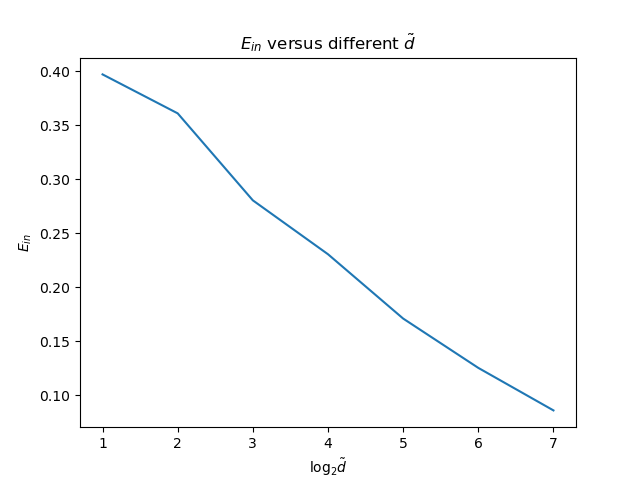
\includegraphics[scale = 0.65]{p11.png}
        \end{center}
        
        \newpage
        \item We can see that in this problem, $E_{in}$ are all the same (small, actually) under second-degree polynomial kernel and different $C$. This shows that the complexity of the kernel is suitable for the problem. 
        \begin{center}
            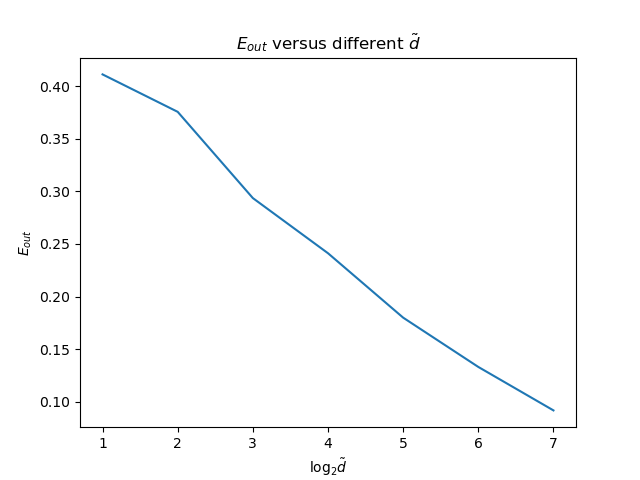
\includegraphics[scale = 0.65]{p12.png}
        \end{center}
        
        \item As $C$ becomes larger, the number of support vectors first grows, then decreases. We guess that because SVM can't find a hyperplane with "fat" margin when the penalty becomes larger, it turns to hyperplanes which is not so "fat". Finding planes with smaller margin would allow more data drop out of the boundary instead of inside the boundary. Hence the number of support vector decrease.
        \begin{center}
            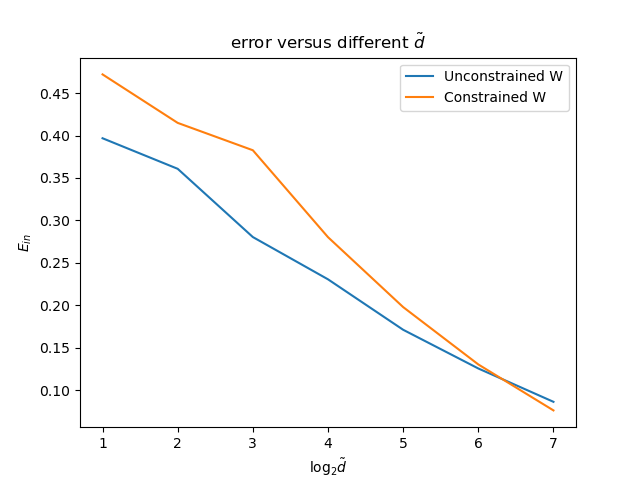
\includegraphics[scale = 0.65]{p13.png}
        \end{center}
        
        \newpage
        \item As $C$ grows, the distance from free support vector to the hyperplane becomes closer. Since we have to avoid the high penalty caused by $C$, it's hard to find a hyperplane with "fat" margin.
        \begin{center}
            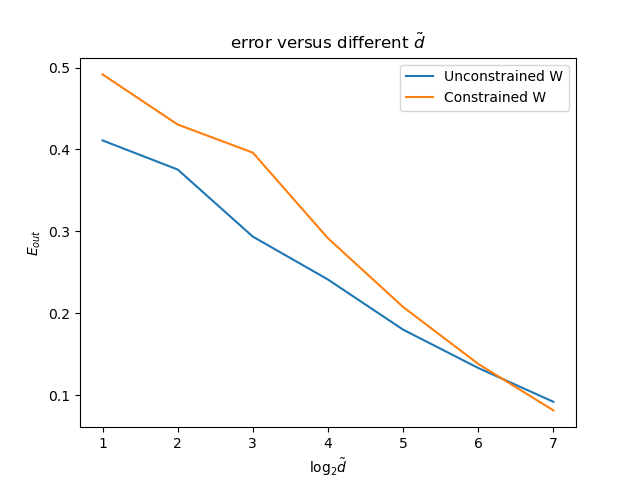
\includegraphics[scale = 0.65]{p14.png}
        \end{center}
        
        \item We can see that $E_{out}$ comes to a minimum when $\gamma = 10$. Higher $\gamma$ may cause overfit, and small $\gamma$ result to underfit.
        \begin{center}
            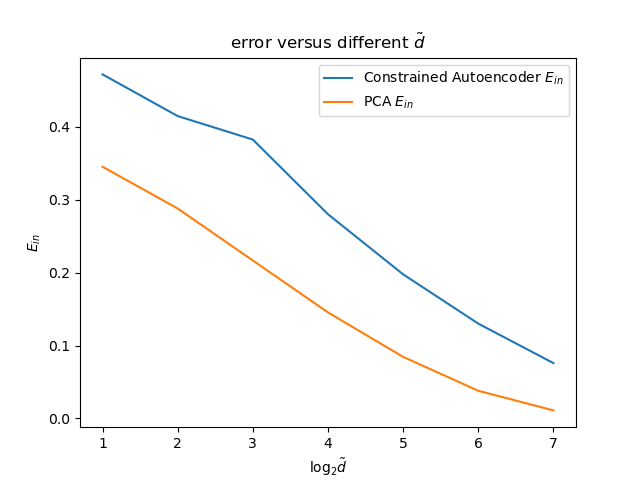
\includegraphics[scale = 0.65]{p15.png}
        \end{center}
        
        \newpage
        \item From the figure, we find that  $\gamma = 10$ is the best choice among the five choice, which has the lowest $E_{val}$. It also meets the result in question 15, which gives that $\gamma = 10$ has the best performance in $E_{out}$.
        \begin{center}
            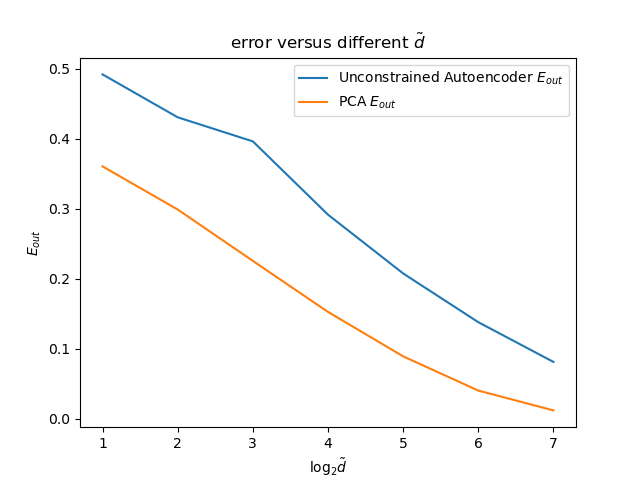
\includegraphics[scale = 0.65]{p16.png}
        \end{center}
        
        \item
        We prove the statement by contradiction.\\
        Assume that there exists a optimal $w_i \neq 0$ for the corresponding feature component $z_i$. Then, we write $(\mathbf{w}^*, b^*)$ with $w_i \neq 0$ is optimal to the problem
        \begin{align*}
            \min_{b, \mathbf{w}}\enspace \enspace& \frac{1}{2}\mathbf{w}^T\mathbf{w}\\
            \text{ subject to }\enspace \enspace& y_n(\mathbf{w}^T\mathbf{z}_n + b) \ge 1
        \end{align*}
        Then, we claim that $(\mathbf{w}', b')$ with $w'_i = 0$ and $w'_j = w^*_j$ for $j \neq i$, and $b' = b^* + w^*_i z_i$ is a better solution to the problem under same constrain.\\
        First we check $(\mathbf{w'},b')$ meets the constraint. For each $n \in \{1, 2, \dots, N\}$, we have
        \begin{align*} \mathbf{w'}^T \mathbf{z}_n + b' = \left(\sum_{k=1}^d w'_k z_{nk}\right) + b' &= \left(\sum_{k=1}^d w'_k z_{nk}\right) + w^*_i z_{ni} + (b' - w^*_i z_{ni}) \\
        &= \mathbf{w^*}^T\mathbf{z}_n + b^* \ge 1 \end{align*}
        Then observe that
        \begin{align*}
            \frac{1}{2}\mathbf{w'}^T\mathbf{w'} = \frac{1}{2}\sum_{k=1}^d (w'_k)^2 &< \frac{1}{2}\sum_{k=1}^d (w^*_k)^2 && \text{ (By $(w^*_i)^2 \ge 0 = (w'_i)^2$) }\\
            &= \frac{1}{2}\mathbf{w^*}^T\mathbf{w^*}
        \end{align*}
        which contradicts to $(\mathbf{w}^*, b^*)$ is optimal. Thus, we end the proof.
        
        \newpage
        \item The dual problem of hard-margin SVM is
        \begin{align*}
            \min\enspace \enspace& \frac{1}{2}\sum_{n=1}^N\sum_{m=1}^N \alpha_n \alpha_m y_n y_m \mathbf{x}_n^T\mathbf{x}_m - \sum_{n=1}^N \alpha_n\\
            \text{ subject to }\enspace \enspace& \sum_{n=1}^N \alpha_n y_n = 0 \text{ and }0\le\alpha_n
        \end{align*}
        Use Lagrange multipliers to "hide" the constraints in the dual problem, we transfer the problem to the form \[\min_{\alpha \in \mathbb{R}^n} \max_{\beta \ge 0, \lambda \ge 0} \mathcal{L}(\alpha, \beta, \lambda)\]
        where 
        \[ \mathcal{L}(\alpha, \beta, \lambda) = \frac{1}{2}\sum_{n=1}^N\sum_{m=1}^N \alpha_n \alpha_m y_n y_m \mathbf{x}_n^T\mathbf{x}_m - \sum_{n=1}^N \alpha_n + \lambda_1(\sum_{n=1}^N \alpha_n y_n) - \lambda_2(\sum_{n=1}^N \alpha_n y_n) - \sum_{i=1}^N \beta_i \alpha_i  \]
        Note that when there's any violating $\alpha$, i.e, $\sum_{n=1}^N \alpha_n y_n \neq 0$ or $\alpha_n < 0$, the Lagrange function would go to $\infty$ by choosing $\beta$, $\lambda_1$ or $\lambda_2$ arbitrary large.
        
        Then, under strong duality, we exchange $\min$ and $\max$
        \[ \max_{\beta \ge 0, \lambda \ge 0}\min_{\alpha \in \mathbb{R}^n}  \frac{1}{2}\sum_{n=1}^N\sum_{m=1}^N \alpha_n \alpha_m y_n y_m \mathbf{x}_n^T\mathbf{x}_m - \sum_{n=1}^N \alpha_n + \lambda_1(\sum_{n=1}^N \alpha_n y_n) - \lambda_2(\sum_{n=1}^N \alpha_n y_n) - \sum_{i=1}^N \beta_i \alpha_i  \]
        Hence the inner problem is unconstrained, we compute $\frac{\partial \mathcal{L}}{\partial \alpha_i}$
        \begin{align*} \frac{\partial \mathcal{L}}{\partial \alpha_i} = \sum_{n=1}^N y_n y_i \alpha_n \mathbf{x_i}^T\mathbf{x_n} - 1 + \lambda_1 y_i - \lambda_2 y_i - \beta_i = 0\\ \Rightarrow \sum_{n=1}^N y_n y_i \alpha_n \mathbf{x_i}^T\mathbf{x_n} = 1 - \lambda_1 y_i + \lambda_2 y_i + \beta_i && (*) \end{align*}
        Then, we know that under optimal $\alpha$,
        \begin{align*}
            \mathcal{L}(\alpha, \beta, \lambda) &= \frac{1}{2}\sum_{n=1}^N\sum_{m=1}^N \alpha_n \alpha_m y_n y_m \mathbf{x}_n^T\mathbf{x}_m - \sum_{n=1}^N \alpha_n + \lambda_1(\sum_{n=1}^N \alpha_n y_n) - \lambda_2(\sum_{n=1}^N \alpha_n y_n) - \sum_{i=1}^N \beta_i \alpha_i\\
            &= \frac{1}{2}\sum_{n=1}^N \alpha_n (1-\lambda_1 y_n + \lambda_2 y_n + \beta_n) - \sum_{n=1}^N \alpha_n + \lambda_1(\sum_{n=1}^N \alpha_n y_n) - \lambda_2(\sum_{n=1}^N \alpha_n y_n) - \sum_{i=1}^N \beta_i \alpha_i\\
            &= -\frac{1}{2}\sum_{n=1}^N \alpha_n (1-\lambda_1 y_n + \lambda_2 y_n + \beta_n)
        \end{align*}
        Hence the "dual of dual" problem becomes
        \begin{align*} \min_{\beta \ge 0, \lambda \ge 0}\frac{1}{2}\sum_{n=1}^N \alpha_n (1-\lambda_1 y_n + \lambda_2 y_n + \beta_n) = \min_{\beta \ge 0, \lambda \ge 0}\frac{1}{2} \alpha^T(\mathbf{1} - \lambda_1 \mathbf{y} + \lambda_2 \mathbf{y} + \mathbf{\beta})
        \end{align*}
        Let $Q$ be an $n \times n$ matrix with $Q_{ij} = y_i y_j \mathbf{x_i}^T\mathbf{x_j}$ and by $(*)$, we have
        \[ \alpha = Q^{-1}(\mathbf{1} - \lambda_1 \mathbf{y} + \lambda_2 \mathbf{y} + \mathbf{\beta}) \]
        Replace $\alpha^T$ with $(\mathbf{1} - \lambda_1 \mathbf{y} + \lambda_2 \mathbf{y} + \mathbf{\beta})^T{Q^{-1}}^T$ we have
        \[\min_{\lambda \ge 0, \beta \ge 0}\frac{1}{2}(\mathbf{1} - \lambda_1 \mathbf{y} + \lambda_2 \mathbf{y} + \mathbf{\beta})^T{Q^{-1}}^T(\mathbf{1} - \lambda_1 \mathbf{y} + \lambda_2 \mathbf{y} + \mathbf{\beta}) \]
        Although it's not the same as the hard-margin SVM primal, but their form are very similar. Both of them are a QP problem with only second-degree coefficient matrix $Q$ in the target function.
    \end{enumerate}
    \end{normalsize}
\end{CJK*}
\end{document}